\documentclass{article}
\usepackage{tikz}
\usetikzlibrary{arrows.meta, positioning, shapes.geometric}
\usepackage{amsmath} % for advanced math environments
\usepackage{amsfonts} % for math fonts
\usepackage{amssymb} % for math symbols
\usepackage{amsthm} % for theorems and proofs
\usepackage{mathtools} % for mathematical tools
\usepackage{mathrsfs} % for script-like fonts in math
\usepackage{bm} % for bold math symbols
\usepackage{bbm} % for "blackboard-style" characters in math
\usepackage{graphicx} % for including graphics
\usepackage{hyperref} % for including hyperlinks
\usepackage{enumitem}
\usepackage{tcolorbox}
\usepackage{tikz}
\tcbuselibrary{theorems, breakable}
\usepackage{xcolor}
\usepackage[margin=1in]{geometry}

\newcommand{\C}{\mathbb{C}}
\newcommand{\N}{\mathbb{N}}
\newcommand{\Q}{\mathbb{Q}}
\newcommand{\R}{\mathbb{R}}
\newcommand{\Z}{\mathbb{Z}}
\newcommand{\pset}{\mathscr{P}}
\DeclareMathOperator{\lcm}{lcm}

% Define a shortcut for \begin{bmatrix} and \end{bmatrix}
\newcommand{\bmat}[1]{\begin{bmatrix}#1\end{bmatrix}}
\newcommand{\cmat}[1]{\begin{pmatrix}#1\end{pmatrix}}

\newtcolorbox[auto counter]{problem}%
{
  breakable,
  colback=cyan!5,
  colframe=cyan!35!black,
  fonttitle=\bfseries,
  title=Problem~\thetcbcounter,
}

\newtcolorbox{solution}[1]
{
  breakable,
  colback=red!5,
  colframe=red!75!black,
  fonttitle=\bfseries,
  title=Solution: #1,
}

% Title
\title{Your Document Title}
\author{Benjamin Basseri}


\begin{document}

\maketitle


\begin{problem}
Let $X$ be a topological space; let $A$ be a subset of $X$. Suppose that for each $x \in A $ there is an open set $U$ containing $x$ such that $U \subset A$. Show that $A$ is open in $X$.
\end{problem}

\textbf{Proof: direct, using the topology axioms and given information}
We're given for each $x \in A$ there is an open set $U$ where $x \in U \subset A$. We have arbitrary unions of open sets are open from the topology axioms. So for each $x$ call the containing open set $U_x$ that is itself contained in $A$, then $A$ is an arbitrary union of open sets, which is open:
$$A = \bigcup_{x \in A} U_x$$

\begin{problem}
Consider the nine topologies on the set $X = \{a, b, c\}$ indicated in Example 1 of \S 12. Compare them; that is, for each pair of topologies, determine whether they are comparable, and if so, which is the finer.
\end{problem}

The first topology is $\mathscr{T}_{\text{trivial}}=\{\varnothing, X\}$, or the 'one big clump' topology. Since all topologies will contain $\varnothing$ and $X$, this topology will be comparable and coarser than all others. Likewise, the last topology is the discrete topology, comparable and finer than all others.

The other topologies are:
$$\mathscr{T}_{\text{nested-}a}=\{\varnothing, \{a\}, \{a, b\}, X\}$$
$$\mathscr{T}_{\text{nested}-b}=\{\varnothing, \{b\}, \{a, b\}, \{b, c\}, X\}$$
$$\mathscr{T}_{\text{isolated}-b}=\{\varnothing, \{b\}, X\}$$
$$\mathscr{T}_{\text{separated}}=\{\varnothing, \{a\}, \{b, c\}, X\}$$
$$\mathscr{T}_{\text{split-}b} = \{\varnothing, \{b\}, \{c\}, \{a, b\}, \{b, c\}, X\}$$
$$\mathscr{T}_{\text{cut-}c} = \{\varnothing, \{a, b\}, X\}$$
$$\mathscr{T}_{\text{closed-}c} = \{\varnothing, \{a\}, \{b\}, \{a, b\}, X\}$$

For $\mathscr{T}_{\text{nested-}a}$ it is only comparable to $\mathscr{T}_{\text{cut-}c}$ and $\mathscr{T}_{\text{closed-}c}$. For the other topologies above it either has $\{a\}$ or $\{a, b\}$ open and the others do not so it is not contained by them, and the others have $\{b\}$ or $\{b, c\}$ open and $\mathscr{T}_{\text{nested-}a}$, so it cannot contain them. This means

$$\mathscr{T}_{\text{trivial}} \subset \mathscr{T}_{\text{cut-}c} \subset \mathscr{T}_{\text{nested-}a} \subset \mathscr{T}_{\text{closed-}c} \subset \mathscr{T}_{\text{discrete}}$$

For the other topologies
$$\mathscr{T}_{\text{trivial}} \subset \mathscr{T}_{\text{isolated}-b} \subset \mathscr{T}_{\text{nested-}b} \subset \mathscr{T}_{\text{split-}b} \subset \mathscr{T}_{\text{discrete}}$$
$$\mathscr{T}_{\text{trivial}} \subset \mathscr{T}_{\text{separated}} \subset \mathscr{T}_{\text{discrete}}$$

\begin{center}
  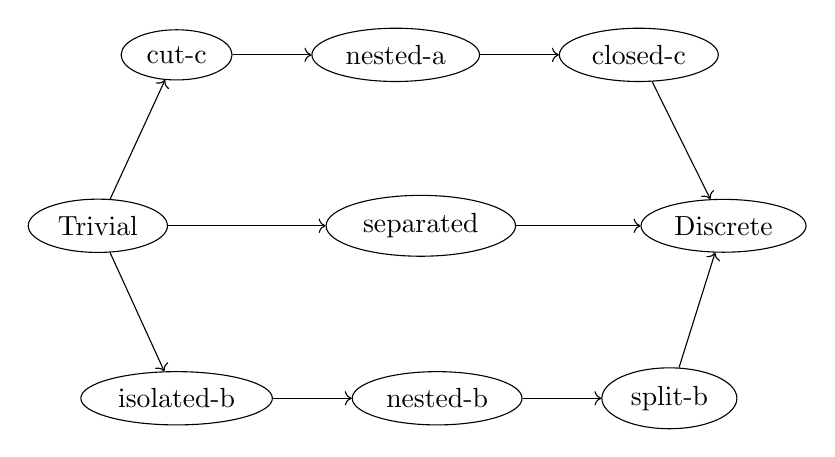
\begin{tikzpicture}[
    node distance=1.5cm and 2cm,
    every node/.style={draw, ellipse, align=center},
    every edge/.style={draw, -{Latex[length=3mm]}}
    ]

    % Nodes
    \node (trivial) {Trivial};
    \node (cutc) [above=of trivial, xshift=1cm] {cut-c};
    \node (nesteda) [above=of cutc, right=of cutc, xshift=-1cm] {nested-a};
    \node (closedc) [right=of nesteda, xshift=-1cm] {closed-c};
    \node (discrete) [right=of trivial, xshift=4cm] {Discrete};

    \node (isolatedb) [below=of trivial, xshift=1cm] {isolated-b};
    \node (nestedb) [right=of isolatedb, xshift=-1cm] {nested-b};
    \node (splitb) [right=of nestedb, xshift=-1cm] {split-b};

    \node (separated) [right=of trivial, xshift=0cm] {separated};

    % Edges
    \draw[->] (trivial) -- (cutc);
    \draw[->] (cutc) -- (nesteda);
    \draw[->] (nesteda) -- (closedc);
    \draw[->] (closedc) -- (discrete);

    \draw[->] (trivial) -- (isolatedb);
    \draw[->] (isolatedb) to (nestedb);
    \draw[->] (nestedb) to (splitb);
    \draw[->] (splitb) -- (discrete);

    \draw[->] (trivial) -- (separated);
    \draw[->] (separated) -- (discrete);

  \end{tikzpicture}
\end{center}

\begin{problem}
Show that the colleciton $\mathscr{T}_c$ given in Example 4 of \S 12 is a topology on the set $X$. Is the collection
$$\mathscr{T}_\infty = \{U \mid X - U \text{ is infinite or empty or all of } X\}$$

a topology on $X$?
\end{problem}

Example 4 states: Let $X$ be a set; let $\mathscr{T}_c$ be the collection of all subsets $U$ of $X$ such that $X - U$ is either countable or all of $X$. Check that $\mathscr{T}_c$ satisfies the topology requirements:
\begin{enumerate}
  \item $X - X$ is empty hence countable, so $X \in \mathscr{T}_c$, and $X - \varnothing$ is all of $X$, so $\varnothing \in \mathscr{T}_c$. So $\mathscr{T}_c$ contains $X$ and $\varnothing$.
  \item Suppose you have an arbitrary family of open sets $\{U\}_\alpha$. For each $U_\alpha$ we know $X - U_\alpha$ is countable or all of $X$. If $X - U_\alpha$ is all of $X$ for every $\alpha$, that means each $U_\alpha $ is empty and $\bigcup U_\alpha$ is empty. That makes $X - \bigcup U_\alpha$ all of $X$. Otherwise, there is some $U_\alpha$ where $X - U_\alpha$ is countable. Taking more sets away from $X$ (by unioning them with $U_\alpha$) can only make the result smaller. Also by De Morgan's laws:
        $$ X - \bigcup U_\alpha = \bigcap (X - U_\alpha)$$
        which is an intersection of countable sets and must be countable. Hence the arbitrary union of open sets is open.
  \item Suppose you have a finite family of open sets $\{U\}_n$. By De Morgan's laws:
        $$X - \bigcap_{i=1}^n U_i = \bigcup_{i=1}^n (X - U_i)$$
        Since each $X - U_i$ is countable or all of $X$, the union $\bigcup_{i=1}^n (X - U_i)$ is countable or all of $X$. Hence the finite intersection of open sets is open.
\end{enumerate}

Next we investigate if $\mathscr{T}_\infty$ is a valid topology. $X - X$ is empty and $X - \varnothing$ is $X$ so both $X, \varnothing \in \mathscr{T}_\infty$. However it is possible that the complement of arbitrary unions is not infinite, empty, or $X$. Take $\R$ with the standard topology. Let $U = (-\infty, 0)$ and $V = (0, \infty)$. Then $U, V$ are both open since their complements are infinite, but $\R - (U \cup V) = \{0\}$ which is not infinite, empty, or all of $\R$. Hence $\mathscr{T}_\infty$ is not a topology.

\begin{problem}
\begin{enumerate}[label=\alph*)]
  \item If $\{\mathscr{T}_\alpha\}$ is a family of topologies on $X$, show that $\bigcap \mathscr{T}_\alpha$ is a topology on $X$. Is $\bigcup \mathscr{T}_\alpha$ a topology on $X$?
  \item Let $\{\mathscr{T}_\alpha\}$ be a family of topologies on $X$. Show that there is a unique smallest topology on $X$ containing all the collections $\mathscr{T}_\alpha$, and a unique largest topology on $X$ contained in all $\mathscr{T}_\alpha$.
  \item If $X = \{a, b, c\}$, let
        $$\mathscr{T}_1 = \{\varnothing, \{a\}, \{a, b\}, X\} \text{ and } \mathscr{T}_2 = \{\varnothing, X, \{a\}, \{b, c\}\}$$
        Find the smallest topology containing $\mathscr{T}_1$ and $\mathscr{T}_2$, and the largest topology contained in $\mathscr{T}_1$ and $\mathscr{T}_2$.
\end{enumerate}

\end{problem}

\begin{enumerate}[label=\alph*)]
  \item Since every set in the family is a valid topology, they all contain $X$ and $\varnothing$, so these are in the intersection. Then for any family of opens $\{U\}_\beta$ in the intersection, each $U$ is open in every topology so their arbitrary union is in each member topology and hence in the intersection. The same goes for finite intersections. Hence the intersection of the family of topologies is a topology.

        The union of topologies might not be a topology since you could have a $U$ open in one topology and $V$ open in another but their union or intersection might not be in the union of topologies. Let $X = \{a, b\}$ and suppose you have topologies $\{\{a\}, \varnothing, X\}$ and $\{\{b\}, \varnothing, X\}$. Then $\{a\}$ is open in the first and $\{b\}$ is open in the second, but $\{a, b\}$ does not belong to either topology so it's not in their union.

  \item The smallest topology containing all the collections $\mathscr{T}_\alpha$ is the one with $\bigcup \mathscr{T}_\alpha$ as a subbasis $\mathscr{S}$. First, closing $\mathscr{S}$ under finite intersections adds the finite intersection requirement, as we may have $U$ open in one $\mathscr{T}_\alpha$ and $V$ open in another, but not having both of them in the same topology which would guarantee their intersection be present. For example you could have $\mathscr{T}_1, \mathscr{T}_2$ from part c; the first topology contains $\{a, b\}$ and the second contains $\{b, c\}$, but their intersection $\{b\}$ is not in the union. After closing on finite intersections it's now a basis but it may still lack some open sets as we just saw. So closing it under unions clears the arbitrary union requirement. Now you have a basis that generates a topology containing all $\mathscr{T}_\alpha$.

        To show this is the smallest possible topology, let $\mathscr{T}$ be the topology generated by $\bigcup \mathscr{T}_\alpha$ and assume towards a contradiction that there was a topology $\mathscr{T}'$ that contained $\bigcup \mathscr{T}_\alpha$ but was strictly contained in $\mathscr{T}$. Then there is some $U \in \mathscr{T}$ that doesn't belong to $\mathscr{T}'$. This $U$ can be written as a union of basis elements from $\bigcup \mathscr{T}_\alpha$, but $\mathscr{T}'$ is supposed to contain all those basis elements as well; so it is lacking an arbitrary union and can't be a valid topology.

        The largest topology contained in all $\mathscr{T}_\alpha$ is the intersection of all $\mathscr{T}_\alpha$. We know this is a valid topology and is contained in each $\mathscr{T}_\alpha$. To show this is the largest possible topology contained in the intersection, if there was a topology $\mathscr{T}'$ strictly larger than $\mathscr{T} = \bigcap \mathscr{T}_\alpha$ then $\mathscr{T}'$ has some $U$ that is not in $\mathscr{T}$. But this means $U$ is not in some $\mathscr{T}_\alpha$ for some $\alpha$, which means $\mathscr{T}'$ is not contained in the intersection.

  \item As just shown, the smallest topology containing both topologies is \textit{generated} by their union as a subbasis, and the largest topology containing them is their intersection. The union:
        $$\mathscr{T}_1 \cup \mathscr{T}_2 = \{\varnothing, \{a\}, \{a, b\}, \{b, c\}, X\}$$

        Closing this set under finite intersections adds $\{b\} = \{a, b\} \cap \{b, c\}$. Closing under unions doesn't add any additional sets making the topology generated by $\mathscr{T}_1 \cup \mathscr{T}_2$:
        $$\mathscr{T}_1 \vee \mathscr{T}_2 = \{\varnothing, \{a\}, \{b\}, \{a, b\}, \{b, c\}, X\}$$

        The largest topology containing both topologies is their intersection:
        $$\mathscr{T}_1 \cap \mathscr{T}_2 = \{\varnothing, \{a\}, X\}$$
\end{enumerate}

\begin{problem}
Show that if $\mathscr{A}$ is a basis for a topology on $X$, then the topology generated by $\mathscr{A}$ equals the intersection of all topologies on $X$ that contain $\mathscr{A}$. Prove the same if $\mathscr{A}$ is a subbasis.
\end{problem}

\textbf{Basis proof: inclusion both ways.}

Let $\mathscr{T}(\mathscr{A})$ be the topology generated by $\mathscr{A}$ and $\{\mathscr{T}_\alpha\}$ be the family of all topologies containing $\mathscr{A}$. For the forward inclusion, consider that $\mathscr{T}(\mathscr{A})$ is generated by including all unions in $\mathscr{A}$. Any topology containing $\mathscr{A}$ must contain all these unions as well, so any $U \in \mathscr{T}(\mathscr{A})$ must be in every $\mathscr{T}_\alpha$, and hence in the intersection. Therefore $\mathscr{T}(\mathscr{A}) \subset \bigcap \mathscr{T}_\alpha$. For the reverse inclusion, $\mathscr{T}(\mathscr{A})$ is a topology containing $\mathscr{A}$ and so a member of $\{\mathscr{T}_\alpha\}$; intersecting it with other topologies cannot make it bigger and $\bigcap \mathscr{T}_\alpha \subset \mathscr{T}(\mathscr{A})$.

\text{Subbasis proof: inclusion both ways.}

Much the same as before, if $\mathscr{A}$ is a subbasis the the topology it generates $\mathscr{T}(\mathscr{A})$ must contain all finite intersections and unions of them. Any topology containing $\mathscr{A}$ must contain all these finite intersections and unions as well, so any $U \in \mathscr{T}(\mathscr{A})$ must be in every $\mathscr{T}_\alpha$, and hence in the intersection. Therefore $\mathscr{T}(\mathscr{A}) \subset \bigcap \mathscr{T}_\alpha$. For the reverse inclusion, $\mathscr{T}(\mathscr{A})$ is a topology containing $\mathscr{A}$ and so a member of $\{\mathscr{T}_\alpha\}$; intersecting it with other topologies cannot make it bigger and $\bigcap \mathscr{T}_\alpha \subset \mathscr{T}(\mathscr{A})$.

\begin{problem}
Show that the topologies of $\R_\ell$ and $\R_K$ are not comparable.
\end{problem}

\textbf{Proof: find a set open in each but not the other.}

The set $[a, b)$ is open in $\R_\ell$ but not in $\R_K$. To find a set open in $\R_K$ but not $\R_\ell$ consider than near 0, any interval $(-a, a) - K$ lacks an infinite number of $K$ terms. So $(-a, a) - K$ is open in $\R_K$, but
    $$(-a, a) - K = (-a, 0] \cup (0, a) -K$$
  While it may be possible to decompose $(0, a)$ to an arbitrary union between each $(\frac{1}{n+1}, \frac{1}{n})$, it would then have to be unioned with $(-a, 0]$ which is not open in $\R_\ell$. Hence the topologies are not comparable.

  \begin{problem}
  Consider the following topologies on $\R$:
  \begin{align*}
    \mathscr{T}_1 & = \text{ the standard topology}                                                          \\
    \mathscr{T}_2 & = \text{ the topology of } \R_\ell                                                       \\
    \mathscr{T}_3 & = \text{ the finite complement topology}                                                 \\
    \mathscr{T}_4 & = \text{ the upper limit topology, having all sets } (a, b] \text{ as basis}             \\
    \mathscr{T}_5 & = \text{ the topology having all sets } (-\infty, a) = \{x \mid x < a\} \text{ as basis}
  \end{align*}

  Determine, for each of the following topologies, which of the others it contains.
  \end{problem}

  To give the symbols more memorable subscripts, refer to them as:

  \begin{align*}
    \mathscr{T}_{\R}        & = \text{ standard topology} = \R \text{ with the standard topology} \\
    \mathscr{T}_{\ell}      & = \R_\ell \text{ lower limit topology}                              \\
    \mathscr{T}_{\text{FC}} & = \text{ finite complement topology}                                \\
    \mathscr{T}_u           & = \text{ upper limit topology}                                      \\
    \mathscr{T}_{lt}        & = \text{ topology with basis } (-\infty, a)
  \end{align*}

  For starters we know the lower limit topology is strictly finer than the standard topology on $\R$. Prove that the lower limit is finer by comparing bases: a topology is strictly finer than another if for every basis element $B$ in the coarser topology and any $x \in B$, there is a basis element $B'$ in the finer topology containing $x$. For any basis element $a, b)$ in the standard topology and any $x \in (a, b)$, the basis element $[x, b) \in \R_\ell$ is contained in $(a, b)$. However for any basis element $[a, b) \in \R_\ell$, to capture $a$ in a standard basis element $(a-x, a+y)$ would have to extend below $a$ and include elements outside of $[a, b)$, so it can't be contained in $[a, b)$ making the lower limit strictly finer. Therefore $\mathscr{T}_{\R} \subset \mathscr{T}_{\ell}$.

  Next, compare the lower limit topology $\mathscr{T}_\ell$ to the finite complement topology $\mathscr{T}_{\text{FC}}$. Here we can compare the topologies directly as sets. If $U \in \mathscr{T}_{\text{FC}}$ and $U^c$ is $X$ then $U = \varnothing$, which is in any topology. Otherwise, for $U$ with a finite complement, order the missing elements as $x_1, \ldots, x_n$. Then $U$ can be written as:
$$U = X - \{x_1, \ldots, x_n\} = (-\infty, x_1) \cup (x_1, x_2) \cup \ldots \cup (x_{n-1}, x_n) \cup (x_n, \infty)$$

  The lower limit topology does have open intervals as open sets, since it is strictly finer than $\R$ and contains its open sets (or consider any open interval is the arbitrary union of $(a + 1/k, b)$ starting at a sufficiently large $k$). So $U \in \mathscr{T}_{\text{FC}} \implies U \in \mathscr{T}_\ell$ and the lower limit topology is finer than the finite complement topology. Checking if it's strictly finer, consider that a basis element $[a, b)$ in the lower limit topology has an infinite complement and thus not open in $\mathscr{T}_{\text{FC}}$. Therefore $\mathscr{T}_{\text{FC}} \subset \mathscr{T}_\ell$.

  Next compare $\mathscr{T}_\R$ to $\mathscr{T}_{\text{FC}}$. Similarly to the previous comparison, take any $U$ open in the finite complement. If $U^c = X$ then $U = \varnothing$ and $U \in \mathscr{T}_{\R}$. Otherwise, $U$ has a finite complement and can be written as a union of open intervals, which is also in $\mathscr{T}_{\R}$ making the finite complement coarser than the standard topology. Furthermore, $(a, b)$ is open in $\mathscr{T}_{\R}$ but has an infinite complement so it's not open in $\mathscr{T}_{\text{FC}}$, making the standard topology strictly finer than the finite complement topology. So after comparing the first three topologies we have:
$$\mathscr{T}_{\text{FC}} \subset \mathscr{T}_{\R}  \subset \mathscr{T}_\ell$$

  Next compare the upper limit topology $\mathscr{T}_u$ to the lower limit topology $\mathscr{T}_\ell$ using the bases. With basis element $[a, b)$, target $a$. There is no basis element $(a-x, a+y]$ that can capture $a$ without extending below $a$ and thus not be contained in $[a, b)$ Similarly, for $b$ in $(a, b]$ no basis element of the form $(b-x, b+y]$ can capture $b$ without extending above $b$. Therefore these topologies aren't comparable. However, just as the lower limit topology is strictly finer than the standard topology, the upper limit is strictly finer than $\mathscr{T}_\R$ as well using the same proof.

  Finally, compare the last topology to the others. Since $\mathscr{T}_\R$ has all these same basis elements this implies $\mathscr{T}_{lt}$ is coarser. Checking this topology if it can also be finer than $\mathscr{T}_\R$, consider an arbitrary union $(-\infty, \alpha)$ for an arbitrary collection of $\alpha$'s. The resulting set has the form $(-\infty, \beta)$ where $\beta$ is the supremum of the $\alpha$'s. Similarly, with the intersection $(-infty, a) \cap (-\infty, b)$ the result is $(-\infty, \min(a, b))$, and likewise with any finite intersection. Therefore all open sets in $\mathscr{T}_{lt}$ have the form $(-infty, x)$ and there are any basis element in the standard topology $(a, b)$ is not open in $\mathscr{T}_{lt}$, making the standard topology strictly finer and $\mathscr{T}_{lt} \subset \mathscr{T}_\R$.

  All that remains is to compare $\mathscr{T}_{lt}$ to the finite complement topology $\mathscr{T}_{\text{FC}}$. Write a set $U$ with finite complement as $U = X - \{x_1, \ldots, x_n\}$. Then $U$ can be written as:
$$U = (-\infty, x_1) \cup (x_1, x_2) \cup \ldots \cup (x_{n-1}, x_n) \cup (x_n, \infty)$$

This open set cannot belong to $\mathscr{T}_{lt}$ since it doesn't have the form $(-\infty, x)$, so $\mathscr{T}_{\text{FC}} \not\subset \mathscr{T}_{lt}$. Likewise an open set $(-\infty, x)$ in $\mathscr{T}_{lt}$ has an infinite complement and is not open in $\mathscr{T}_{\text{FC}}$, so $\mathscr{T}_{lt} \not\subset \mathscr{T}_{\text{FC}}$ and the two topologies are not comparable.

\begin{center}
  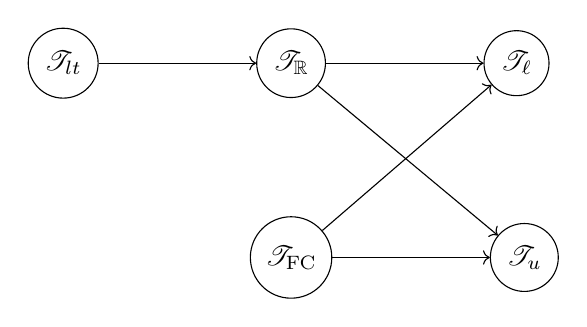
\begin{tikzpicture}[
    node distance=1.5cm and 2cm,
    every node/.style={draw, circle, align=center},
    every edge/.style={draw, -{Latex[length=3mm]}}
    ]

    % Nodes
    \node (lt) {$\mathscr{T}_{lt}$};
    \node (R) [right=of lt] {$\mathscr{T}_\R$};
    \node (l) [right=of R] {$\mathscr{T}_\ell$};
    \node (FC) [below=of R] {$\mathscr{T}_{\text{FC}}$};
    \node (u) [right=of FC] {$\mathscr{T}_u$};

    % Edges
    \draw[->] (lt) -- (R);
    \draw[->] (R) -- (l);
    \draw[->] (R) -- (u);
    \draw[->] (FC) -- (l);
    \draw[->] (FC) -- (u);



  \end{tikzpicture}
\end{center}

\begin{problem}
\begin{enumerate}[label=\alph*)]
  \item Apply Lemma 13.2 to show that the countable collection
        $$\mathscr{B} = \{(a, b) \mid a < b, a, b \in \Q\}$$
        is a basis that generates the standard topology on $\R$.
  \item Show that the collection
        $$\mathscr{C} = \{[a, b) \mid a < b, a, b \in \Q\}$$
        is a basis that generates a topology different from the lower limit topology on $\R$.
\end{enumerate}
\end{problem}

\begin{enumerate}[label=\alph*)]
  \item Lemma 13.2 states that a collection $\mathscr{B}$ is a basis if for every $U$ open in $X$ and each $x \in U$ there is some $B \in \mathscr{B}$ such that $x \in B \subset U$. So take any $U$ open in $\R$; represented as a union of open intervals. Then for any interval $(a, b)$ if the endpoints are rational then it is in the set $\mathscr{B}$ described in the problem setup. Otherwise, WLOG suppse $a$ is irrational. Then construct a sequence of rationals $(a_n) \to a$ and the union $\bigcup (a_n, b)$ will contain any $x \in (a, b)$ and itself be contained in $(a, b)$. Therefore this is a basis for $\R$ and in fact corresponds to the standard basis.
  \item There are two ways you can look at this. First, consider that these basis elements while restricted to rational endpoints can still union to any open interval with rational or irrational endpoints. For any target endpoints $a$ and $b$, construct sequences of rationals $(a_n) \to a$ where all $a_n \in (a, b)$ and $(b_n) \to b$ with all $b_n \in (a, b)$. Then the union

        $$\bigcup [a_n, b_n) = (a, b)$$

        This indicates that this basis generates the standard topology on $\R$, which is strictly coarser than the lower limit topology and hence cannot be the same topology.

        The other way is to compare the basis direclty to the lower limit topology. For any basis element in the lower limit $[a, b)$ with irrational $a$, it's impossible to form a basis element in $\mathscr{C}$ that contains $a$ and is contained in $[a, b)$. This is impossible because any half-open interval with rational endpoints cannot start at $a$, which is irrational, so it must start at some $a - x$ which is lower than $a$ and necessarily will contain elements not in $[a, b)$, and hence not be contained in $[a, b)$. Therefore the basis $\mathscr{C}$ generates a topology different from the lower limit topology.

\end{enumerate}


\end{document}

\end{document}
